\section{Testkvalitet, Coverage og BVA}

Man kan skrive tusindvis af test, men antallet af tests betyder ikke at systemet er bedre testet. 

Når tests skal skrives vil vi gerne gøre det på den mest effektive måde. Vi vil gerne være hurtigt færdige og samtidigt vide at alt er testet.\\

Til dette bruger vi diverse former for \textit{coverage} og \textit{boundary value analyser}.

\subsection{Coverage}
Er en structural test-teknik, som kan bruges ved både unit- og integrationstest. En høj coverage procent sikrer dog ikke at ens test er af høj kvalitet, men bruges til at sikre at man har 'dækket' koden fuldstændigt. Der findes fire typer:

\subsubsection{Function coverage} 
Ser om alle metoder er kørt under test.

\subsubsection{Statement/Line coverage} 
Er alle statements blevet eksekveret (return, call, assignment)? 

\begin{align*}
	Line Coverage \% = \frac{Source Lines Reached By Test}{Lines Of Source Code}
\end{align*}

\vskip.34cm

Ulempen ved dette er at testen er \textit{whitebox}. Yderligere er den insensitiv overfor kontrolstrukture, den tester altså ikke om begge scenarier af et if-statement bliver kørt.

\subsubsection{Branch/Decision coverage}
Er alle branches blevet kørt? Er alle \textit{boolean}'s blevet evalueret til både \textit{true} og \textit{false} i f.eks. while, switch og if? Altså om systemet er testet ud af ''alle stier''.

\subsubsection{Condition coverage}
Beskriver hvorvidt alle \textit{boolean sub-expressions} er evalueret til både \textit{true} og \textit{false}. I Code listing~\ref{code:coverage} er $x > 0$ og $y > 0$ eksempler på \textit{sub-expressions}.

\vskip.4cm

\begin{lstlisting}[caption=Eksempel til div. coverage typer.,label=code:coverage]
int Foo(int x, int y)
{
	int z = 0;	
	
	if( x > 0 && y > 0)
	{
		z = x;
	}
	
	return z;
}
\end{lstlisting}

Med udgangspunkt i Code listing~\ref{code:coverage} beskrives de forskellige former for coverage herunder.

\begin{itemize}
	\item[\textbf{Function}] Hvis metoden \textit{Foo()} bliver kaldt under test er denne opfyldt.
	\item[\textbf{Line}] Med \textit{Foo(1,1)} vil denne være opfyldt, da alle linjer/statements 'rammes'.
	\item[\textbf{Branch}] Ved \textit{Foo(1,1)} og \textit{Foo(1,0)} vil denne være opfyldt. Da begge 'veje' gemmen metoden testes.
	\item[\textbf{Condition}] Her er det nødvendigt med \textit{Foo(1,1)}, \textit{Foo(1,0)} og\textit{Foo(0,0)}, da $x$ og $y$ begge skal evalueres til både \textit{true} og \textit{false} under test.
\end{itemize}

Det vigtigt at være opmærksom på at man godt kan opfylde \textbf{condition coverage} uden at opfylde \textbf{branch coverage}. Ved eksemplet i Code listing~\ref{code:coverage} vil \textit{Foo(1,0)} og \textit{Foo(0,1)} opfylde condition, med ikke branch coverage.

\subsection{Boundary Value Analysis}
Hvis vi har følgende kode, vist i Code listing~\ref{code:bva}. Det er en metode som kan beslutte om et tal er positivt eller negativt.

\begin{lstlisting}[caption=Eksempel til BVA og EP.,label=code:bva]
public bool IsPositive(int number)
{
	if(number > -1)
	{
		return true;
	}		
	return false;
}
\end{lstlisting}

For koden vist overfor, vil dens \textit{equivalence partitions} se ud som vist på figur~\ref{fig:ep}. Her vil alle tal under 0 være $EP_1$ og alle over eller lig 0 være $EP_2$. For eksemplet kan vi så finde \textit{lower valid/invalid boundary} og \textit{upper valid/invalid boundary} for \textbf{begge} EP'er.

\begin{figure}[h]
\centering
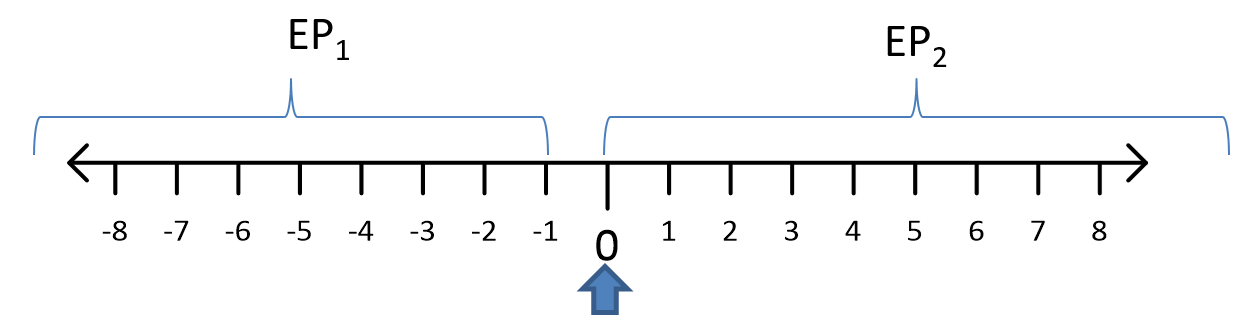
\includegraphics[width=\linewidth]{figs/ep}
\caption{Equivalence partitions, for \textit{IsPositive()}.}
\label{fig:ep}
\end{figure}

Da der ikke er nogen øvre grænse for positive tal eller nedre grænse for negative tal, vil vi kun finde \textit{\textbf{upper} valid/invalid boundary} for $EP_1$ og \textit{\textbf{lower} valid/invalid boundary} for $EP_2$. Disse vil så være som vist herunder:

\begin{table}[H]
	\centering
	\begin{tabular}{lclc}
		%\toprule
		\rowcolor{Black!25} $EP_1$ 		&				& $EP_2$ 		&			\\ %\midrule
		Upper valid						&$~~=-1$			& Lower valid	& $=0$		\\
		Upper invalid 					&$=0$			& Lower invalid	& $~~=-1$		\\ %\hline
		\rowcolor{Black!5} Lower valid	&$~~~~= -\infty$	& Upper valid 	&$~= \infty$ \\ %\bottomrule
	\end{tabular}
	\caption{Boundary values for Code listing~\ref{code:bva}. Med $EP_1$ Lower og $EP_2$ Upper i lysegrå.}
\end{table}

















